\documentclass{article}

\usepackage{hyperref}
\usepackage{amsmath}
\usepackage{bm}
\usepackage{amssymb}
\usepackage{amsfonts}
\usepackage{amstext}
\usepackage{graphicx}

\title{\textbf{Extended Kalman Filter for Fixed-Wing Aircraft Dynamics}}
\author{\textbf{Ahmed M. Hassan}\thanks{am.hassan89@gmail.com}}

\begin{document}

\maketitle

\section{Introduction}
The goal of this project is to implement an extended Kalman filter (EKF) to estimate
a fixed-wing aicraft state vector from noisy sensor measurments. 
The first iteration of this project will be focused only on the longitudinal dynamics.
   
\section{Aircraft Model}
The nonlinear longitudinal dynamics for conventional fixed-wing aircraft can be written as follows \cite{Nelson, Stevens-Lewis}
\begin{equation}\label{Eq:Nonlinear_sys}
    \begin{split}
        \dot{U} &= -Q W - g \sin{\theta} + \frac{X}{m}\\
        \dot{W} &= Q U + g \cos{\theta} + \frac{Z}{m}\\
        \dot{Q} &= \frac{M}{I_{yy}}\\
        \dot{\theta} &= Q
    \end{split}
\end{equation}
The forces and moments can be broken down as follows
\begin{equation}
    \begin{split}
        X &= q S \biggl(C_X(\alpha) + \frac{\bar{c}}{2 V_T} C_{X_Q} Q + C_{X_{\delta_e}} \delta_e\biggr) +
        X_{t_0} + X_{\delta_t} \delta_t\\
        Z &= q S \biggl(C_Z(\alpha) + \frac{\bar{c}}{2 V_T} C_{Z_Q} Q + C_{Z_{\delta_e}} \delta_e\biggr)\\
        M &= q S \bar{c} \biggl(C_M(\alpha) + \frac{\bar{c}}{2 V_T} C_{M_Q} Q + C_{M_{\delta_e}} \delta_e \biggr)
    \end{split}
\end{equation}
Considering a trim condition in a cruise level flight, the nonlinear system \ref{Eq:Nonlinear_sys} 
can be further simplified to be on the following from
%This nonlinear model is very simple and has only very few nonlinear terms-need to have a more sophisticated model later
\begin{equation}\label{Eq:Nonlinear_sys_cruise}
    \begin{split}
        \dot{U} &= -Q W - g \cos{\theta_0} \Delta \theta+ X_U \Delta U + X_W \Delta W +
                 X_{\delta_e} \delta_e + X_{\delta_t} \delta_t\\
        \dot{W} &= Q U - g \sin{\theta_0} \Delta \theta + Z_U \Delta U + Z_W \Delta W + Z_{\delta_e} \delta_e\\
        \dot{Q} &= M_U \Delta U + M_W \Delta W + M_Q Q + M_{\delta_e} \delta_e + M_{\delta_t} \delta_t\\
        \dot{\theta} &= Q
    \end{split}
\end{equation}

The nonlinear system \ref{Eq:Nonlinear_sys} can be linearized and
written in a standard linear system form as follows \cite{Nelson, Stevens-Lewis}
\begin{equation} \label{Eq:Linearized_sys}
    \begin{bmatrix}
    \dot{U} \\
    \dot{W} \\
    \dot{Q} \\
    \dot{\theta} \\ 	
    \end{bmatrix}
    =
    \begin{bmatrix}
    X_u & X_w & 0 & -g \cos{\theta_0}\\
    Z_u & Z_w & U_0 & -g \sin{\theta_0}\\
    M_u & M_w & M_q & 0\\
    0 & 0 & 1 & 0 \\
    \end{bmatrix}
    \begin{bmatrix}
    U \\
    W \\
    Q \\
    \theta \\ 	
    \end{bmatrix}
    +
    \begin{bmatrix}
    X_{\delta_e} & X_{\delta_t} \\
    Z_{\delta_e} & 0 \\
    M_{\delta_e} & M_{\delta_t} \\
    0 & 0\\ 	
    \end{bmatrix}
    \begin{bmatrix}
    {\delta_e} \\
    {\delta_t}  	
    \end{bmatrix}
\end{equation}

In this project we will consider the longitudinal model of the aircraft "DELTA" given in \cite[PP. 561--563]{Mclean}
whose parameters are given as follows (at $U_0 = 75~ m/s$ and $\theta_0 = 2.7 ^\circ$)
\begin{equation}\label{Eq:DELTA_Params}
    \begin{split}
        m &= 300000 kg\\
        X_U &= -0.02\\
        X_W &= 0.1\\
        Z_U &= -0.23\\
        Z_W &= -0.634\\
        M_U &= -2.55*10^{-5}\\
        M_W &= -0.005\\
        M_Q &= -0.61\\
        X_{\delta_e} &= 0.14\\
        Z_{\delta_e} &= -2.9\\
        M_{\delta_e} &= -0.64\\
        X_{\delta_t} &= 1.56\\
        M_{\delta_t} &= 0.0054\\
    \end{split}
\end{equation}
where $\delta_t$ is considered to be from the trim thrust. 
As such, $\delta_t$ is allowed the between $1$ and $-0.56$ \cite{Hassan2016_JAST}.  

\section{Extended Kalman Filter Equations}
In this section, we will summarize the continous-discrete EKF equations as presented by Crassidis and Junkins \cite{Junkins}.
The EKF considers a nonlinear system with process and measurment noise as follows
\begin{equation}
    \begin{split}
        \dot{\bm{x}}(t) &= \bm{f}(\bm{x}(t), \bm{u}(t), t) + G(t) \bm{w}(t),~ \bm{w}(t) \sim N(0, Q(t))\\
        \widetilde{\bm{y}}_k &= \bm{h}(\bm{x}_k) + \bm{v}_k,~ \bm{v}_k \sim N(0, R_k)
    \end{split}
\end{equation}
where the overscript symbol $\widetilde{}$ denotes a measured quantity and the subscript symbol $_k$ denotes the value at time step $k$. 
Also, $\bm{x}$ is the state vector, $\bm{u}$ is the control input vector, $\bm{w}$ is the process noise vector, and $\bm{v}$ is the measurment noise vector.

The EKF can be initialized as follows
\begin{equation}
    \begin{split}
        \hat{\bm{x}}(t_0) &= \hat{\bm{x}}_0\\
        P_0 &= E\{\widetilde{\bm{x}}(t_0) \widetilde{\bm{x}}^T(t_0)\}
    \end{split}
\end{equation}
where the overscript symbol $\hat{}$ denotes an estimated quantity and $P$ is the state estimate error covariance matrix.

The Kalman gain, updated state, and updated state estimate error covariance can be obtained as follows
\begin{equation}
    \begin{split}
        K_k &= P_k^- C_k^T \biggl(C_k P_k^- C_k^T + R_k\biggr)^{-1}\\
        C_k &\equiv \frac{\partial \bm{h}}{\partial \bm{x}}\bigg|_{{\hat{\bm{x}}}_k^-}\\
        \hat{\bm{x}}_k^+ &= \hat{\bm{x}}_k^- + K_k \biggl(\widetilde{\bm{y}}_k - \bm{h}(\hat{\bm{x}}_k^-)\biggr)\\
        P_k^+ &= \biggl(I - K_k C_k\biggr) P_k^-
    \end{split}
\end{equation}
where the superscript symbol $^-$ denotes the state/covariance after the propagation step but before the update step. 
On the other hand, the superscript symbol $^+$ denotes the state/covariance after the update step.

Finally, the state and state estimate error covariance can be propagated as follows
\begin{equation}
    \begin{split}
        \dot{\bm{x}}(t) &= \bm{f}(\bm{x}(t), \bm{u}(t), t)\\
        \dot{P}(t) &= A(t) P(t) + P(t) A^T(t) + G(t) Q(t) G^T(t)\\
        A(t) &\equiv \frac{\partial \bm{f}}{\partial \bm{x}}\bigg|_{\hat{\bm{x}}(t), \bm{u}(t)}
    \end{split}
\end{equation}

\section{Algorithm Structure}
Figure \ref{Fig:EKF_Algorithm_Sketch} shows a simple sketch of the algorithm structure. 
There are two classes implemented in this project: \textit{LongDynamics} and \textit{EKF}. 
The first one encapsulates the nonlinear dynamic system equations for the fixed-wing aircraft longitudinal dynamics, 
whereas the second one encapsulates the EKF algorithm implementation. The \textit{LongDynamics} class relies on an external 
package (odeint \cite{odeint_website}) for time propagation (numerical integration). 
In addition, there are some helper functions to load the dataset and compute the root mean square error.
\begin{figure}[h]
    \centering
    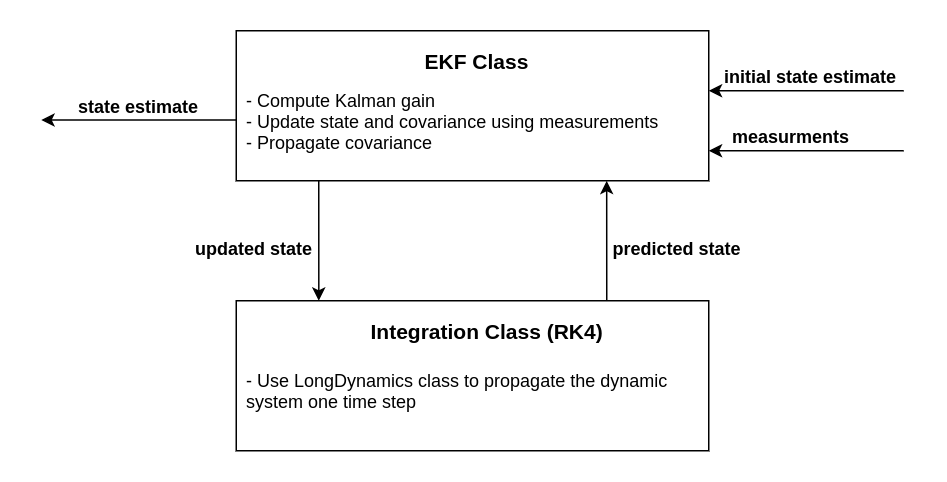
\includegraphics[width=0.9\textwidth]{EKF_Algorithm.png}
    \caption{EKF algorithm structure.}
    \label{Fig:EKF_Algorithm_Sketch}
\end{figure}

\section{Results}
Figures \ref{Fig:Results_AoA} and \ref{Fig:Results_pitchRate} show the estimated angle of attack and pitch rate versus the measured and true ones.
\begin{figure}[h]
    \centering
    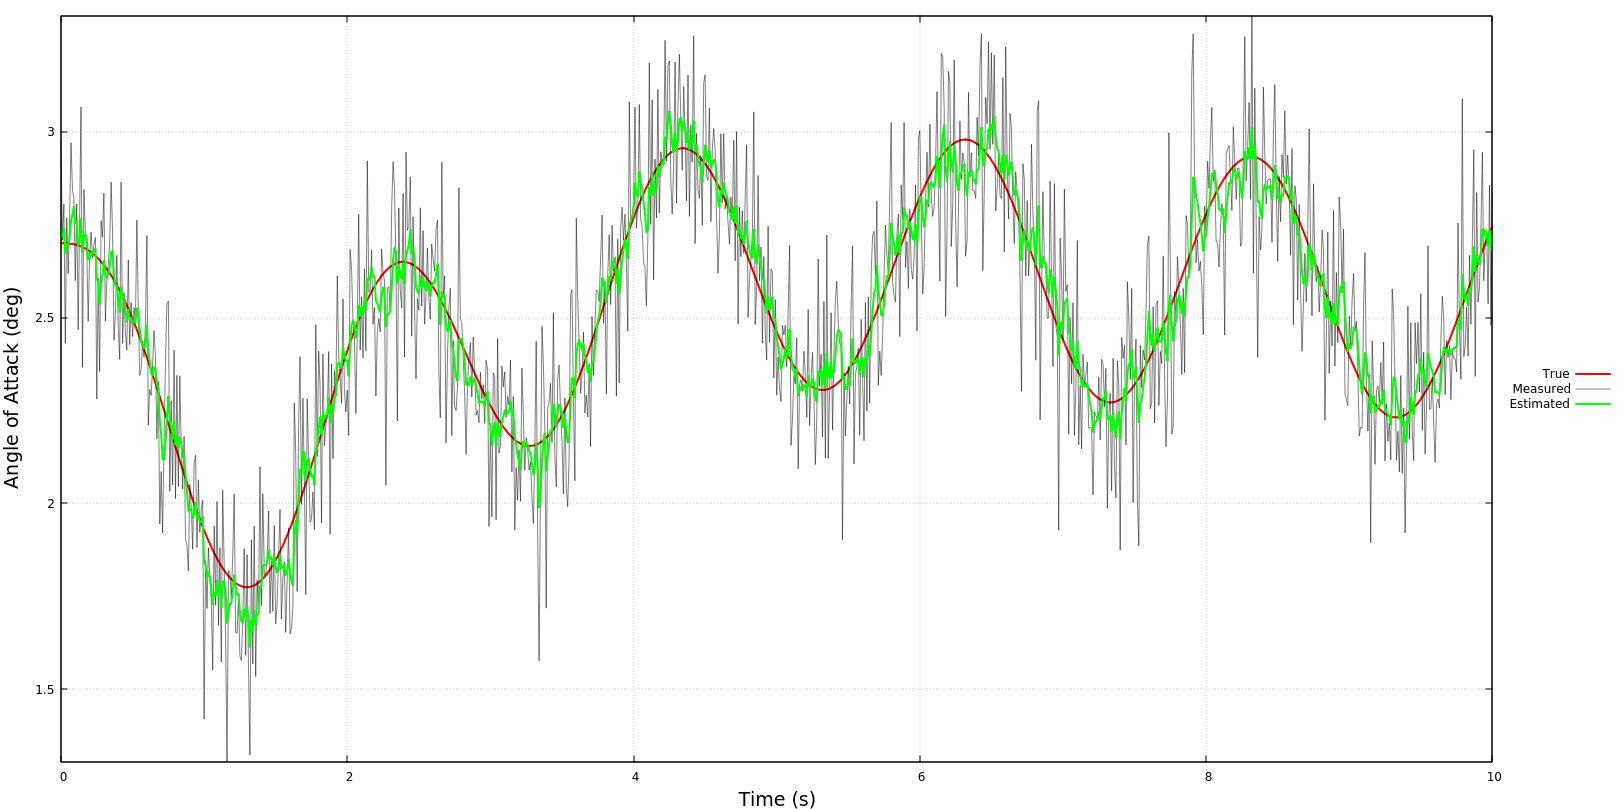
\includegraphics[width=0.9\textwidth]{results_AoA.png}
    \caption{A comparison between the estiamted, measured and true angle of attack.}
    \label{Fig:Results_AoA}
\end{figure}
\begin{figure}[h]
    \centering
    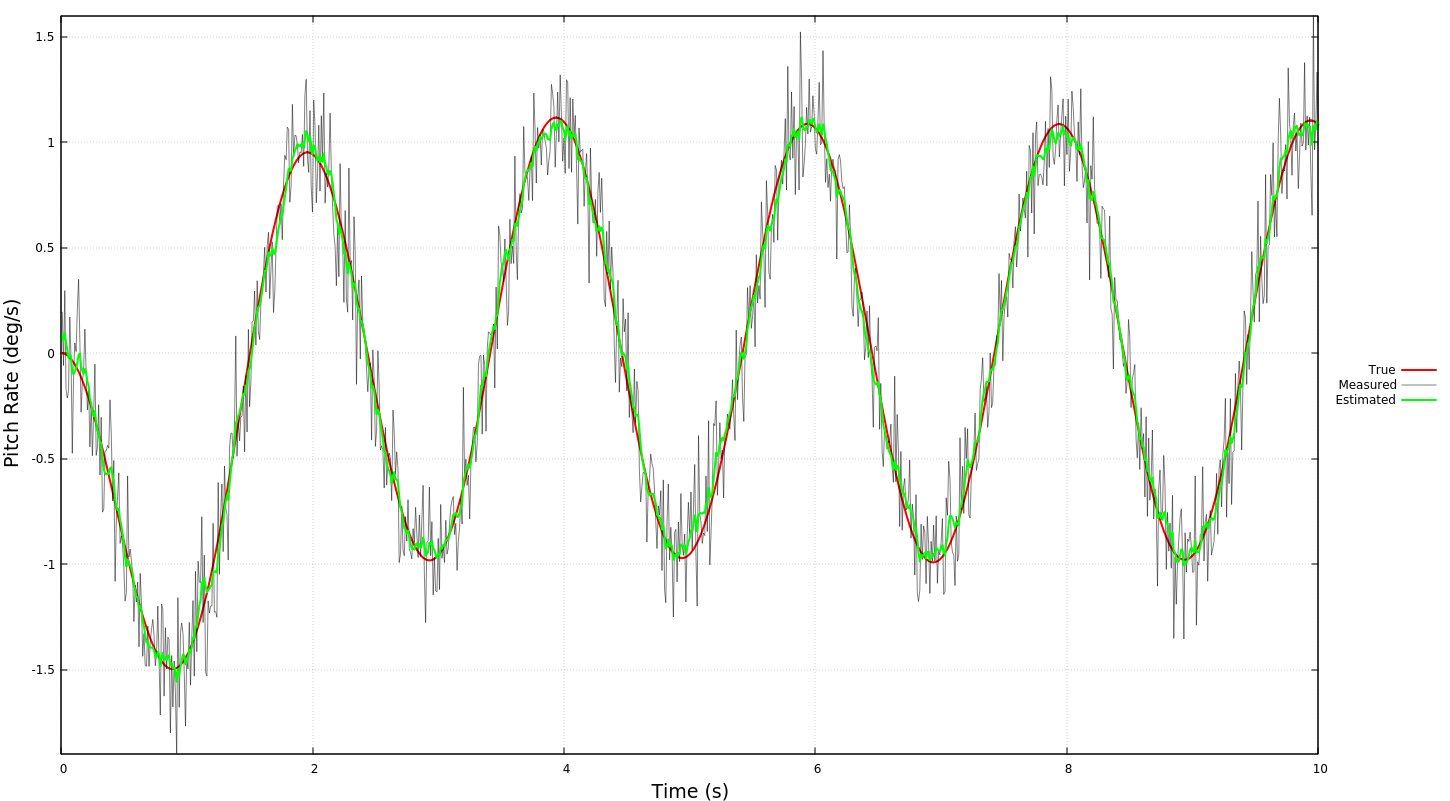
\includegraphics[width=0.9\textwidth]{results_q.png}
    \caption{A comparison between the estiamted, measured and true ptich rate.}
    \label{Fig:Results_pitchRate}
\end{figure}

\bibliographystyle{unsrt}
\bibliography{ref}
\end{document}